\documentclass{cernatsnote}
\usepackage{siunitx}
\usepackage[table,xcdraw]{xcolor}
%\usepackage[colorinlistoftodos]{todonotes}
\usepackage{placeins}
\usepackage{titlesec}
\usepackage{subfigure}
\usepackage{float}
\usepackage{booktabs}
\setcounter{secnumdepth}{4}
\setcounter{tocdepth}{4}    %
\usepackage{amssymb}
\usepackage{url}

\usepackage{booktabs}
\usepackage{multirow}
\usepackage{rotating,tabularx}
\usepackage{tikz}
\usetikzlibrary{patterns}

\titleformat{\paragraph}
{\normalfont\normalsize\bfseries}{\theparagraph}{1em}{}
\titlespacing*{\paragraph}
{0pt}{3.25ex plus 1ex minus .2ex}{1.5ex plus .2ex}

%%%%%%%%%%%%%%%% TITLE PAGE %%%%%%%%%%%%%%%% 
    \title{CHIMERA November 2022 Report}
    \author{
    	To be completed \; \\		
    	CERN, CH-1211 Geneva, Switzerland
    }
    \date{\today}
    \keywords{}
    \begin{document}
    \newcommand{\figref}[1]{Fig.\,\ref{#1}}
    \newcommand{\tabref}[1]{Table\,\ref{#1}}
    \newcommand{\secref}[1]{Section\,\ref{#1}}

    \maketitle
    
    \begin{abstract}
        \ldots
    \end{abstract}
%%%%%%%%%%%%%%%% TITLE PAGE END %%%%%%%%%%%% 

    \begingroup
    \color{black}
    \pagebreak
    \tableofcontents
    \endgroup

\pagebreak

\section{Introduction} %all
\begin{figure}[!htb]
\centering
\includegraphics[width=1.0\textwidth]{images/CCC_eastt8_small.png}
\caption{The CERN accelerator complex. The path of the lead ion beam used by CHIMERA is highlighted in color.}
\label{fig:CCC}
\end{figure}

\section{Beam properties - PS configuration and T8 beam instruments}
% as set in the PS and measured by the beam instruments

\subsection{Proton Synchrotron beam energy} % Eliott
% Some intro about how it is defined, including the lookup tables
% The nice colour showing which energy was used during each moment of the test
The Proton Synchrotron (PS) is a crucial component of the accelerator complex, responsible for accelerating particles from the Proton Synchrotron Booster (PSB) to the Super Proton Synchrotron (SPS) and ultimately to the Large Hadron Collider (LHC). Additionally, the PS is capable of receiving and accelerating heavy ions from the Low Energy Ion Ring (LEIR) for extraction to the East Area, making it a versatile machine. RF cavities are used to accelerate charged particles, such as protons or Pb ions, to high energies, while 100 dipoles bend the beam around the PS's 628 m circumference \cite{gilardoni_fifty_2011}. The particles are then extracted using slow extraction through a beam line and transported to the CHARM facility, which houses the CHIMERA instruments.
\\

The beam energy refers to the kinetic energy per nucleon $E_{kin}$ of the charged particle beam. For an ion beam, the total kinetic energy, denoted $E_{kin, TOT}$, can be obtained by multiplying $E_{kin}$ by the atomic mass number $A$ (where $A = Z + N$, representing the total number of protons $Z$ and neutrons $N$ in the ion).  The total momentum for an ion beam is \cite{chao_handbook_2013}

$$pc={E_{0}\sqrt{\gamma^{2}-1}}$$

$$pc = E_{0}\sqrt{\left [ \left( \frac{E_{kin, TOT}}{E_{0}}+1\right )^{2}-1\right ]}$$

where, $E_{0}$ is the rest mass of the ion and $\gamma=\frac{E}{E_{0}}=\frac{E_{0}+E_{kin}}{E_{0}} = \frac{E_{kin}}{E_{0}}+1$
\\

CHIMERA uses a lead ion beam. During acceleration, the beam is a Pb54+ ion beam of partially stripped electrons (which means that it has 28 $e^{-}$ remaining and thus 54 charges) of isotope A=208.
\\

\begin{figure}
    \centering
    \begin{minipage}{0.45\textwidth}
        \centering
        \includegraphics[width=1.0\textwidth]{images/PS_BEAM_ENERGY/vaccum_window.jpg}
        \caption{Vacuum window connecting the PS to the transfer line leading to the East Area.}
        \label{fig:vaccum window}
    \end{minipage}\hfill
    \begin{minipage}{0.45\textwidth}
        \centering
        \includegraphics[width=1.0\textwidth]{images/PS_BEAM_ENERGY/stripping.jpg} 
        \caption{Diagram illustrating the stripping process, where an ion loses its remaining electrons. The resulting ion has a higher charge state when it travels through the transfer line.}
        \label{fig:stripping}
    \end{minipage}
\end{figure}

As an example for a 1 GeV per nucleon, the momentum would be:

$$pc = E_{0}\sqrt{\left [ \left( \frac{1\text{ [GeV]}\cdot 208}{E_{0}}+1\right )^{2}-1\right ]}$$
where the rest mass $E_{0}$ of Pb54+ is:

$$E_{0} = m_{Pb54+}= 82\cdot m_{proton} + 126\cdot m_{neutron} + 28\cdot m_{e^{-}} - m_{defect} = 193.74 \frac{\text{GeV}}{\text{c}^{2}}$$

with mass defect; see Table \ref{table:masses}: $m_{defect}=82\cdot m_{proton} + 126\cdot m_{neutron} + 28\cdot m_{e^{-}} - 208\cdot m_{u}$ 

\begin{table}[h!]
\centering
\begin{tabular}{lr}
\toprule
Particle & mass GeV/$\text{c}^{2}$\\
\midrule
$m_{proton}$ & 0.93828      \\
$m_{neutron}$ & 0.93957      \\
$m_{e^{-}}$ & 0.000511 \\
$m_{u}$ & 0.9315       \\
\bottomrule
\end{tabular}
\caption{Rest masses \cite{boston_university_nuclear_nodate}.}
\label{table:masses}
\end{table}

The equation that links beam momentum to rigidity in Tesla meter is: 
$$B\rho \text{ [T m]} = 3.3356\cdot p/q \text{ [GeV/c]}$$
where for the PS, $\rho = 70.0789$ m. This formula is used to calculate the bending B-field in the PS dipoles.
\\

For the ESA run, three energies were chosen: 1000, 750 and 650 MeV/nucleon, and the associated magnetic field (B-field) required were calculated, as shown in Fig. \ref{fig:lookup table} and Table \ref{table:KE_table}. Since the ion beam is partially stripped in the PS and becomes fully stripped after passing through the exit vacuum window in the F61 transfer line located after the first quadrupole Q74L, two different rigidities are required for acceleration and transport, respectively. The magnets in the transfer line must be pulsed with a rigidity appropriate for the newly fully stripped ion beam. Significant effort has been invested in automating the scaling of magnets in F61 and the T8 transfer line. A makerule is used to compute the correct strength to apply based on the PS B-field (and thus beam energy). The makerule computes a partially stripped momentum for the first quadrupole in F61 and a second momentum for a fully stripped ion beam for the rest of the transfer line down to CHARM. This automatic scaling is highly advantageous, as energy scans can be performed by simply adjusting the B-field at flat-top of the PS. However, some limitations exist, such as the need for occasional manual corrections to the extraction path and SMH57 and SMH61, as well as the fact that the bending to the East Dump has not yet been associated with a makerule (only the current can be adjusted).

\begin{figure}[!htb]
\centering
\includegraphics[width=1.0\textwidth]{images/PS_BEAM_ENERGY/kinetic_energy_lookup_chimera.png}
\caption{Lookup table for the lead ion beam flat-top in the Proton Synchrotron (PS). The magnetic field required for acceleration to three different energies (1000, 750, and 650 MeV/nucleon) as well as energy scan measurements to the East Dump is shown.}
\label{fig:lookup table}
\end{figure}

\begin{table}[h!]
\centering
\begin{tabular}{rrrrl}
\toprule
 $E_{kin}$ [MeV/nucleon] &  $\frac{pc}{54}$ [GeV] &  $\frac{pc}{82}$ [GeV] &  PS B-field [G] & USER\\
\midrule
  1000 &                        6.517 &                    4.292 &        3102 & CPS.USER.EAST4 \\
   750 &                        5.392 &                    3.551 &        2566 & CPS.USER.EAST3 \\
   650 &                        4.923 &                    3.242 &        2343 &   CPS.USER.MD5 \\
\bottomrule
\end{tabular}
\caption{Table showing the kinetic energy used during the ESA November 2022 run. The term 'USER' refers to the settings the PS is loaded with. A USER profile saves all magnet strengths, which can be easily accessed and applied to the PS when that particular USER is called, similar to a preset configuration.}
\label{table:KE_table}
\end{table}

Figure \ref{fig:bfield} illustrates the magnetic field profile of the main dipoles in the Proton Synchrotron (PS) produced by the PS main magnet Power system (POPS). The profile includes two distinct regions - the injection plateau where protons are injected from LEIR, and the flat-top extraction plateau where protons have achieved maximum energy and are ready for extraction. Note that the spike at the end, which was introduced to overcome certain limitations of POPS, is irrelevant to the extraction process and can be disregarded.

\begin{figure}[!htb]
\centering
\includegraphics[width=0.6\textwidth]{images/PS_BEAM_ENERGY/average_b_field_chimera.png}
\caption{CHIMERA's magnetic field at different energies, with injection plateau at 684 G and extraction plateau at varying B-field strengths corresponding to different energy levels.}
\label{fig:bfield}
\end{figure}

During the CHIMERA ion run in November, the experiment lasted for 5 days, from Wednesday the 23rd of November afternoon to Monday morning the 28th of November at 6 o'clock in the morning. The energies used during the run were 1000, 750, and 650 MeV/nucleon and were used for almost the same amount of time. The 650 MeV/nucleon was used for 36\% of the time, the 750 MeV/nucleon was used for 28\%, and the 1000 MeV/nucleon was used for 35\%. The run was divided into specific tasks and timeframes, see Fig. \ref{fig:timestamp_energies}. Wednesday and Thursday were used for beam preparation, Friday and Saturday were devoted to ESA's experiment, and Sunday was used for backup or for additional machine development. During the first few hours of the beam time, the focus was on characterizing the three energies and varying intensity as per the standard beam instruments. The next few hours were dedicated to testing all four DUTs sequentially for all energies, followed by a run overnight to accumulate statistics on the Renesas memory. On Thursday morning, the team had the option to either change to a second degrader thickness or another set of DUTs, or do a "degrader scan." Friday and possibly part of Saturday were dedicated to ESA's experiment. The rest of Saturday night and Sunday were left for backup and for optics measurements.

\begin{figure}[!htb]
\centering
\includegraphics[width=1.0\textwidth]{images/PS_BEAM_ENERGY/user_mapping_timestamp.png}
\caption{Timestamps of beam energies: the plot displays the time stamps associated with different beam energies used during the November run.}
\label{fig:timestamp_energies}
\end{figure}

Following the ESA run, an automatic script was used to ramp the beam energy for further development purposes. A dedicated energy scan was conducted on the diode using 5 different beam energies, ranging from 775 MeV/u to 900 MeV/u. A separate experiment was carried out to measure the lowest beam energy that could be recorded at the East Dump, which was found to be 283 MeV/nucleon. The main limitation was that the bending magnet to the dump is not scaled with momentum, and hand corrections were needed to propagate the beam to the dump, as well as the beam spot on the BTV being large and weak at this energy, which made observation difficult. Lower energies could be tried out in the future.


\begin{figure}
    \centering
    \begin{minipage}{0.45\textwidth}
        \centering
        \includegraphics[width=1.0\textwidth]{images/PS_BEAM_ENERGY/energy_scan_chimera 1.png}
        \caption{Plot of the B-field showing different flat-tops during an energy scan.}
        \label{fig:energy_scan}
    \end{minipage}\hfill
    \begin{minipage}{0.45\textwidth}
        \centering
        \includegraphics[width=1.0\textwidth]{images/PS_BEAM_ENERGY/energy_scan_timestamp_chimera 1.png} 
        \caption{Energy scan with timestamp.}
        \label{fig:energy_scan_timestamp}
    \end{minipage}
\end{figure}

% \subsection{Beam intensity} \label{beam_intensity} % Eliott, Kacper
% RFKO and gain settings throughout the test
% Intensity measurements on SEC and XION, including intensity vs. gain
%%%%%%%%%%%%%%%%%%
%%%%%% RFKO %%%%%%
%%%%%%%%%%%%%%%%%%
\subsection{Slow extraction - RFKO}

The ion slow extraction scheme uses the magnetic septums SMH57 and SMH61 to extract the beam to the East Area. Unlike the proton slow extraction, in the case of the lead ion beam, the electrostatic septum SEH23 is bypassed as its entry and exit windows would strip the ions from the remaining electrons, which would change the rigidity during extraction; see Fig. \ref{fig:sx}.

\begin{figure}[!htb]
\centering
\includegraphics[width=0.4\textwidth]{images/BEAM_INTENSITY/SX_CHIMERA.jpg}
\caption{Pb-ion beam slow extraction scheme}
\label{fig:sx}
\end{figure}

To jump the septum, the required amplitude growth is achieved through the use of bumps and third-order integer slow extraction. The standard slow extraction technique in the PS involves shrinking a third-order integer triangle formed by separatrices (produced by a non-linear field) by changing the horizontal betatron tune (Qx). Iterations of the scheme were performed, beginning with a ramp on the low-energy quadrupoles (LEQ) to increase the tune to the third integer resonant tune. However, a different slow extraction scheme using Radiofrequency Knock Out (RFKO) was ultimately adopted during the 2022 November run to improve the control of the beam intensity at different energies. In RFKO, the beam is slowly extracted due to emittance growth induced by a transverse RF-field at a third of the revolution frequency. The resonance line serves as a threshold above which the particles become unstable. The RF-frequency is modulated over time (using frequency modulation, or FM, close to a third of the revolution frequency), with a frequency sweep (or chirp) performed to affect off-momentum particles. The chirping signal increases the beam emittance and diffuses the particles from the beam core to the stable triangle, see Fig. \ref{fig:steinbach_diagram} and \ref{fig:rfko}. The frequency sweep ensures that a large fraction of the particles in the beam are kicked and start the diffusion process. As the machine does not ramp, the stable triangle remains fixed in phase-space during the extraction \cite{noda_slow_1996, badano_proton-ion_1999, dulla_radio_2019}.
\\

\begin{figure}
    \centering
    \begin{minipage}{0.45\textwidth}
        \centering
        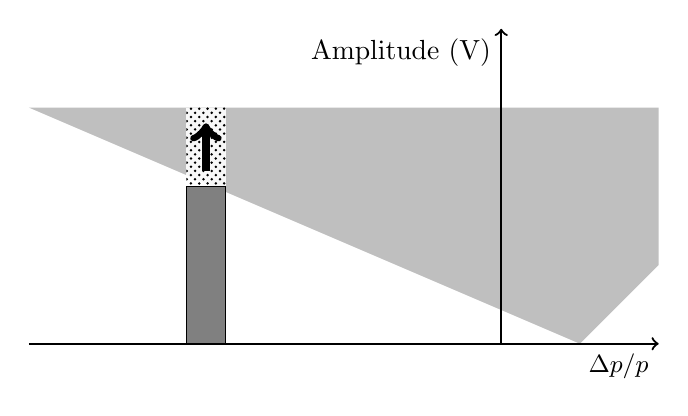
\begin{tikzpicture}
            \path [fill=lightgray] (1,0) -- (-6,3) -- (2,3) -- (2,1) -- (1,0);
        	\draw [->, thick] (-6,0) -- (2,0) node [below left] {\small$\Delta p/p$};
        	\draw [->, thick] (0,0) -- (0,4)  node [below left] {Amplitude (V)};
         % Waiting stack
            \draw[fill=gray] (-4,0) rectangle (-3.5,2);
         % Extracted beam
            \fill[fill=white, fill opacity=0.9] (-4,2) rectangle (-3.5,3);
            \fill[fill=gray, fill opacity=1.0, pattern = crosshatch dots] (-4,2) rectangle (-3.5,3);
        \draw [->, line width = 1mm] (-3.75,2.2) -- (-3.75,2.8);
        \end{tikzpicture} 
        \caption{In RFKO, transverse stochastic noise or RF excitation at the revolution frequency is used to excite the beam and induce growth in its betatron amplitudes.}
        \label{fig:steinbach_diagram}
    \end{minipage}\hfill
    \begin{minipage}{0.45\textwidth}
        \centering
        \includegraphics[width=1.0\textwidth]{images/BEAM_INTENSITY/RFKO.jpg}
        \caption{The emittance growth diffuses the particles from the beam core to the unstable triangle.}
        \label{fig:rfko}
    \end{minipage}
\end{figure}

The RFKO setup involved using the radial loop GRPOS to bring the beam's tune close to resonance, followed by a slight backing off from the resonance using the same radial loop. This was preferred over using the low-energy quadrupoles (LEQ), which also changes the tune but also the optics. Once the target tune was attained, the radial loop was turned off and the beam was debunched. The optics of the machine remained static, without any ramping. The Transverse Feedback Blowup (TFB) was then employed to push particles into resonance with the help of the the Q-meter software to chirp the beam. At low frequencies, the chirps were visible in the spill, but for faster chirping $< 1$ ms, the frequencies were high enough to be mostly suppressed by the transit time. For more details on the beam time structure, see section \ref{beam_time_structure}.

%%%%%%%%%%%%%%%%%%%%%%%%%%%%
%%%%%% BEAM INTENSITY %%%%%%
%%%%%%%%%%%%%%%%%%%%%%%%%%%%
\subsection{Beam intensity}
\label{beam_intensity}



The RFKO scheme has different parameters to control the extraction:
\begin{enumerate}
    \item Chirp gain: the voltage applied to the RFKO plates.
    \item Chirp frequency range
    \item Accuracy (number of turns in the PS)
    \item Bounds: Start and stop of the chirping
\end{enumerate}

Lowest chirps is 512 turns
Time it takes for one turn in the PS = **2.1 $\mu s$**
* $t = \frac{circumference}{c} = \frac{628}{3e8} = 2.1e-6 [s]$

5.12e2 * 2.1e-6 = 1.752e-3 s = 1.8 ms

\begin{figure}[!htb]
\includegraphics[width=1.0\textwidth]{images/BEAM_INTENSITY/flux_vs_gain.png}
\end{figure}


Additionally, the smallest beam area with the constraints on power converter amperage of 733, 537 and 421 A respectively is simulated to be 0.904 mm.




\subsection{Spill time profile} % Eliott
% Gas scintillator, SEC, XION, etc.
% Diode SMU measurements could be included here, even if introduced later
Understanding the time profile of a beam spill is crucial for various reasons in accelerator physics and radiation testing of electronic devices. One key aspect is the flux, which refers to the number of particles per square centimeter per second (p/cm²·s) that pass through a device over a given period of time. A high flux of particles during a spill can lead to a high number of Single Event Effects (SEE) in electronic devices under test, which can degrade and fail sooner than if they were exposed to a lower flux over the same period of time. In radiation testing, a constant flux is preferred to simplify the analysis, however, a non-uniform spill with an accurate time profile and flux measurement as a function of time is also useful. This chapter will present a detailed analysis of the time profile of the slow extracted spills that occurred during the November 2022 run. The analysis will include a description of the instruments and methods used to gather data, a presentation of the results, and a discussion of the implications of these results for future beams.

\subsubsection{Instruments and location}

Seven instruments are used to measure the time profile. These are the gas scintilator, the Secondary Emission Chambers (XSECs) (23/70/94), the Ionization Chamber XION(71/94) and the diode. The numbers refer to the position of the instrument in the transfer line in a sequential order. The instruments in position 94 are the closest to the device under test.

The Beam Current Measurement based on Gas (BCGAA), previously known as a longitudinal spill detector (LSD), utilizes nitrogen gas to detect beam-induced ionization photons. The collected photons generate an electric signal, which is then amplified and sampled using a photo-multiplier (PM) to accurately measure the beam current.

The XSECs are used to measure the number of particles passing through the accelerator. They work by directing the beam through a series of thin metal foils, such as aluminum. When the beam interacts with the foils, it generates secondary electrons which are then detected by a charge-integrating circuit. The integrated current is proportional to the number of particles passing through the foils and is often converted into counts for ease of data transmission. XSECs have varying sensitivities depending on their design and number of foils. For instance, in the T08 beamline, T08.XSEC070 (which has 10 foils) has a sensitivity four times higher than T08.XSEC094 (which only has 2 foils) \cite{ravotti_calibration_2022}.

An example of the spill time profile of the XSEC70 is shown in Fig. \ref{fig:spill_time_profile1}.

\begin{figure}[!htb]
\centering
\includegraphics[width=0.6\textwidth]{images/spill_profile_xsec_CPS.USER.EAST3_0.1_1.png}
\caption{Single spills are plotted in gray and the average of the spills in plotted in blue.}
\label{fig:spill_time_profile1}
\end{figure}

\begin{figure}[!htb]
\centering
\includegraphics[width=0.6\textwidth]{images/bar_chart_gain_energy.png}
\caption{Spill time profile}
\label{fig:spill_time_profile2}
\end{figure}

\begin{figure}[!htb]
\centering
\includegraphics[width=0.6\textwidth]{images/spill_profile_xsec70_average_EAST3.png}
\caption{Spill time profile}
\label{fig:spill_time_profile3}
\end{figure}

\begin{figure}[!htb]
\centering
\includegraphics[width=0.6\textwidth]{images/spill_profile_xsec70_average_gain_0.1.png}
\caption{Spill time profile}
\label{fig:spill_time_profile4}
\end{figure}

\subsubsection{Beam Time Structure}
\label{beam_time_structure}

The beam under study displays a complex frequency structure, with slow and fast frequencies present. To deliver a slow extracted beam, the Radio Frequency Knock Out (RFKO) technique is employed. This involves generating a chirp waveform with a predetermined repetition rate. However, in 2022, the Qmeter2 software that controls the voltage on the RF plates limited the maximum chirp repetition rate to 1 millisecond intervals, see Fig. \ref{fig:RFKO_chirp_explanation}. As a result, a spectral line at 1 kHz is produced. Additionally, a fast spill structure is observed at the fractional tune of the third integer, corresponding to frev/3. The revolution frequencies for the 650, 750, and 1000 MeV beams are 385, 397, and 417 kHz, respectively, resulting in spectral lines at approximately 130 kHz and their associated harmonics. The gas scintillator used for detection has a Nyquist frequency of 1 kHz due to its 0.5 ms sampling rate, capturing only the lowest frequency lines. Conversely, the diode's much faster sampling rate of 0.5 $\mu$s enables it to detect both slow and fast frequencies, as seen in Fig. \ref{fig:spill_fft_diode}. Future runs could benefit from adjusting the sampling granularity to be coarser or finer, down to the nanosecond scale.

\begin{figure}[!htb]
\centering
\includegraphics[width=1.0\textwidth]{images/SPILL_TIME_PROFILE/RFKO_chirp_explanation.jpg}
\caption{The RF chirps at a repetition rate of 1 kHz during a chirp length. Although a chirp length that is not a power of 2 would be more optimal for our needs, we are currently forced to use a power of 2 by design of the Qmeter2 software that controls the voltage on the RF plates. As shown in the diagram, the RF frequency ramps up during the chirp and repeats the ramping at every chirp, producing a quasi sawtooth signal. This signal blows up the emittance and extracts the beam.}
\label{fig:RFKO_chirp_explanation}
\end{figure}

\begin{figure}[!htb]
\centering
\includegraphics[width=0.9\textwidth]{images/SPILL_TIME_PROFILE/CHIMERA_diode_FFT_two_scales.png}
\caption{FFT of a 650 MeV spill at 0.15 gain measured with the diode in CHARM. The left plot shows the harmonics of the 1 kHz RFKO chirping technique, while the right plot displays the 130 kHz signal and its harmonics.}
\label{fig:spill_fft_diode}
\end{figure}

The fast frequencies are correlated with the revolution frequency of the beam (FREV), which varies with the beam energy, as listed in Table \ref{table:frev}.

\begin{table}[]
\centering
\begin{tabular}{lll}
USER           & frev [kHz] & frev/3 [kHz] \\
\hline
CPS.USER.EAST4 & 417.7      & 139.2        \\
CPS.USER.EAST3 & 397.8      & 132.6        \\
CPS.USER.MD5   & 385.4      & 128.5       
\label{table:frev}
\end{tabular}
\end{table}

During our testing phase, we employed a signal generator to send custom signals to the TFB plates, which could be remotely controlled using Python scripts. However, we did not use it during the November run. To mitigate the impact of low frequencies, we experimented with chirping at a higher repetition rate and pulsing in a continuous sawtooth signal, which effectively damped and broadened the chirp excitation signal. In order to address the higher frequencies induced by the revolution frequency, one idea we are considering is to inject more bunches around the machine and attempt to debunch the beam for longer durations.

\subsection{Beam spatial profile} %Eliott, Kacper
% MWPC, Independence of beam profile with beam intensity, impact of energy on the beam shape, “explanation” of the dips (i.e. comparison with and without Montract), etc.
    \begin{figure}[!htb]
        \centering
        \includegraphics[width=0.48\columnwidth]{images/MWPC/MWPC_horizontal.pdf}
        \includegraphics[width=0.48\columnwidth]{images/MWPC/MWPC_vertical.pdf}
        \caption{Caption}
        \label{fig:my_label}
    \end{figure}
    

\section{Beam properties - solid state detector in DUT position}
% as measured by the silicon diode

\subsection{Setup} % Natalia
% Montrac, cabling, x-y table, degraders/collimators, etc.

% The silicon diode used to asses the characteristics of the CHIMERA heavy-ion beams was a fully depleted passivated implanted planar silicon (PIPS) detector manufactured by Canberra, model \hbox{FD 50-14-300 RM} (denoted as "\textit{Vanessa I}" diode for simplicity). This diode is \SI{308}{\micro\meter} thick and has an active surface of \SI{0.5}{\centi\meter\squared}. This corresponds to the silicon surface in the circular opening of the metal case of the diode with a radius of \SI{111}{\milli\meter}, as it can be seen in Figure~.... A part of the silicon die is also present under the metal case, for a better mechanical stability. The total size of the silicon can reach a radius of up to \SI{13}{\milli\meter}. However, the exact size of the silicon die in this detector was not revealed by the manufacturer and hence, it is not clear how large is the fraction of silicon under the casing also contributing to the particle detection. This diode has an entrance window of $\leq$ \SI{50}{\nano\meter}.

% % To be checked:
% During the test, the diode was wrapped up with two layers of standard commercial \SI{14}{\micro\meter}-thick aluminium foil (i.e.~{\SI{28}{\micro\meter}} of aluminium in front of the diode) to shield it from light and electromagnetic noise.


% The diode was attached to a Plexiglass support plate using a 3D-printed holder, shown in Fig... and the plexiglass plate was attached on the large standard MOMNTRAC frame placed in the most downstream of the three MONTRAC slots.



% % Preapmplifier:
% The diode was used together with a \SI{20}{\deci\bel} current \gls{pa} from Cividec, model C1HV0089. The certified gain of this \gls{pa} is \SI{21.9}{\deci\bel}. The intensity of the beam was high enough, hence no amplification was needed for this test. The \gls{pa} was used for purely practical reasons: to split the detector bias and signal into two separate lines, while they are exiting the diode through a single connector. A \SI{6}{\deci\bel} attenuator was used to partially compensate for this amplification.

% The diode connected to the \gls{pa} with a \SI{20}{\centi\meter}-long cable were both placed on the MONTRAC movable table, as it is shown in Figure X. The \gls{pa} was connected to the rest of the test setup placed outside of the radiation room with three \SI{20}{\meter}-long BNC cables (and the necessary adapters) running through the maze. One BNC cable was used to provide the recommended reverse bias voltage of $+$\SI{200}{\volt} to the detector, supplied by a \gls{smu} Keithley 2410. The second cable was used to power the \gls{pa} with \SI{12}{\volt} DC voltage supplied by another \gls{smu} Keithley 2410 and the third cable was used to transmit the detector signal to the CEAN DT5751 digitizer before being acquired and saved by the acquisition laptop.

\subsection{Diode as a flux monitor} % Kacper
% Including notably the correlation with SEC and XION


\subsubsection{1 GeV/u}
    \begin{figure}
        \centering
        \includegraphics[width=0.48\columnwidth]{images/SEC_XION_DIODE_FLUX/1000.pdf}
        \caption{Caption}
        \label{fig:my_label1}
    \end{figure}

    \begin{figure}
        \centering
        \includegraphics[width=0.48\columnwidth]{images/SEC_XION_DIODE_FLUX/1000_sec.pdf}
        \includegraphics[width=0.48\columnwidth]{images/SEC_XION_DIODE_FLUX/1000_xion.pdf}
        \caption{Caption}
        \label{fig:my_label2}
    \end{figure}
    
\subsubsection{750 MeV/u}
    \begin{figure}
        \centering
        \includegraphics[width=0.48\columnwidth]{images/SEC_XION_DIODE_FLUX/750.pdf}
        \caption{Caption}
        \label{fig:my_label3}
    \end{figure}

    \begin{figure}
        \centering
        \includegraphics[width=0.48\columnwidth]{images/SEC_XION_DIODE_FLUX/750_sec.pdf}
        \includegraphics[width=0.48\columnwidth]{images/SEC_XION_DIODE_FLUX/750_xion.pdf}
        \caption{Caption}
        \label{fig:my_label4}
    \end{figure}

\subsubsection{650 MeV/u}
    \begin{figure}
        \centering
        \includegraphics[width=0.48\columnwidth]{images/SEC_XION_DIODE_FLUX/650.pdf}
        \caption{Caption}
        \label{fig:my_label5}
    \end{figure}

    \begin{figure}
        \centering
        \includegraphics[width=0.48\columnwidth]{images/SEC_XION_DIODE_FLUX/650_sec.pdf}
        \includegraphics[width=0.48\columnwidth]{images/SEC_XION_DIODE_FLUX/650_xion.pdf}
        \caption{Caption}
        \label{fig:my_label6}
    \end{figure}

\subsection{Energy deposition distributions} % Andreas, Natalia
% « Primary » energies, including mysterious energy changes
% Comparison with GSI, which we can consider as calibration/reference
% Impact of degraders
% Impact of collimation
\input{sections/7_Energy_deposition_distributions.tex}

\section{Other measurements}
\subsection{SRAM memories} % Andrea
% SEU counts versus beam intensity
% (note: for actual SEU cross section value/fluence measurements, we would need to accurately know the beam LET, which will in turn likely need to at least partially rely on a combination of simulations and diode measurements. But, we can try to, in first instance, focus on the diode measurements – also because these mysterious energy changes cannot be accounted for in FLUKA, unless understood)
\input{sections/8_SRAM_memories.tex}

\subsection{Scintillator} % Andreas
\input{sections/9_Scintillator.tex}

\newpage
\bibliography{references, references_eliott}
\bibliographystyle{IEEEtran}

\end{document}